\documentclass{article}
\usepackage[utf8]{inputenc}
\usepackage{geometry}
\usepackage[sort]{natbib}
\usepackage{pxfonts}
\usepackage{graphicx}
\usepackage{setspace}
\usepackage{hyperref}
\usepackage{lineno}

\doublespacing
\linenumbers

\title{Episodic memory: mental time travel or a quantum `memory wave' function?}
\author{Jeremy R. Manning\\Dartmouth College, Hanover, NH\\jeremy.r.manning@dartmouth.edu}

\begin{document}
\maketitle

\begin{abstract}
Where do we ``go'' when we recollect our past?  When remembering a past event, it is intuitive to imagine some part of ourselves mentally ``jumping back in time'' to when the event occurred. I propose an alternative view, inspired by recent evidence from my lab and others, as well as by re-examining existing models of episodic recall, that suggests that this notion of mentally revisiting any specific moment of our past is at best incomplete and at worst misleading.  Instead, I suggest that we retrieve information from our past by mentally casting ourselves back simultaneously to \textit{many} time points from our past, much like a quantum wave function spreading its probability mass over many possible states.  This revised conceptual model makes important behavioral and neural predictions about how we retrieve information about our past, and has implications for how we study episodic memory experimentally.
\end{abstract}

\section*{Introduction and overview}
How do our brains organize, retrieve, and act upon the ceaseless flow of incoming information and experiences?  \cite{Tulv83} contends that episodic memory is like a sort of ``mental time travel,'' whereby we send some part of our mental state back along our autobiographical timeline to a specific moment in our past~\citep[also see][]{Tulv72, HassEtal07b, SchaEtal07, MannEtal11}.  This process has also been described as mentally ``jumping back in time''~\citep[e.g.,][]{HowaEtal12, FolkEtal18} to when we experienced what we are now remembering.  This view has fundamental implications for how we study and build theories about memory: it suggests that we can match up specific moments of recollection with specific moments from the past.  These implications extend from how we design episodic memory experiments to how we analyze and interpret the behavioral and neural data from those experiments in order to understand the neural and/or cognitive basis of memory retrieval.  At its core, characterizing episodic memory as mental time travel makes studying and understanding memory about matching.  Specifically, the primary implied questions are about how and when we match up the thoughts (and/or brain activity patterns) we are experiencing at one moment with the thoughts (and/or brain activity patterns) we experienced at another previous moment.  The implied challenge, then, is to understand the neural (structural) and cognitive (functional) mechanisms that characterize when, how, and why our memory systems allow us to relive those prior experiences.  One way of illustrating how this framing misses out on key aspects of memory is to examine how experimentalists and theorists typically conceive of and model a mental construct called \textit{context}.

The notion of context was fundamental to \citeauthor{Tulv83}'s characterization of episodic recall, and continues to be a primary feature of most current theories of episodic memory~\citep[e.g., for review see][]{Kaha12}.  Whereas the \textit{content} of a memory provides specific information about the episode itself, contextual components of a memory help to frame the episode within the rememberer's broader experience.  Defining context precisely (e.g., as distinct from content) is an ongoing challenge for our field, but theorists generally describe context as reflecting a mental combination of external cues (where you are, who you are with, background sensory information, etc.) and internal cues (thoughts, feelings, emotions, etc.) that uniquely define each moment~\citep[e.g., see review by][]{MannEtal15}.  Reactivating the mental representation of the context associated with a given episode is what can give us the feeling of some ``part of ourselves'' re-experiencing the past~\citep[Tulving refers to this feeling as \textit{autonoetic awareness};][]{Tulv02a}.

One practical way to distinguish content from context representations is to separate out mental (or neural) representations that drift rapidly \citep[content;][]{PolyEtal05a, MannEtal12} or gradually \citep[context;][]{PolyEtal05a, MannEtal11, HowaEtal12, LohnEtal18, LongKaha18, FolkEtal18}.  An intuition for why contextual representations might be expected to evolve gradually is laid out by \cite{PolyKaha08}.  Essentially, slowly drifting thoughts may be used to ``index'' more rapidly drifting thoughts that are temporally proximal.  This notion, that our brains maintain parallel mental representations drifting at different timescales, has been well-characterized in a series of elegant fMRI and ECoG studies by Uri Hasson and colleagues~\citep{HassEtal08, LernEtal11, HoneEtal12a, AlyEtal18}.  Subsequent work by the same group has shown that this hierarchy of drifting mental representations plays a central role in how we remember continuous experiences and segment our experiences into discrete events~\citep{BaldEtal17}.  This body of work suggests that different brain regions reflect \textit{temporal receptive windows} that characterize the timescale(s) to which each region is maximally sensitive.  This research complements work on the \textit{temporal window of integration} in the speech and perception literatures~\citep[e.g.,][]{ViemWake91, GautEtal12, vanWEtal07}.  The temporal window of integration refers to the duration over which physically distinct stimuli are treated (by some brain system or network) as a single percept or atomic unit.  This systems-level work mirrors the discovery of \textit{time cells} in the rodent hippocampus that respond preferentially to a specific time relative to a temporal reference (e.g., time elapsed since starting to run on an exercise wheel), whereby each cell appears to integrate incoming information at a different rate~\citep{PastEtal08, MacDEtal11} and the population activity serves to represent information at a range of timescales~\citep{MauEtal18}. Other work suggests that the lateral entorhinal cortex also plays a role in integrating information across a wide range of timescales~\citep{TsaoEtal18}, supporting precise temporal recall~\citep{MontEtal19}.  In addition to this work suggesting that individual systems or neurons maintain representations at their preferred timescales, a number of studies also report neurons and small populations exhibiting \textit{temporal multiplexing}, whereby information at different timescales is reflected in different features of an individual neuron's (or population's) activity patterns, such as spike timing versus firing rate or local field potential oscillations at different frequencies~\citep{CaruEtal18, KnigEich13, WatrEtal13, PanzEtal10}.

The above ideas about parallel neural representations that reflect information at multiple timescales have been formalized in a family of theoretical models over the past several decades~\citep{HowaKaha02a, DianEtal07, SedeEtal08, PolyEtal09, ShanEtal09, ShanHowa10, ShanHowa12, HowaEtal14, Rang18}.  In turn, these models were inspired in part by earlier theoretical work suggesting that temporally proximal experiences become linked through their shared contextual features~\citep{Este55a,AtkiShif68}.  Other recent work indicates that different aspects of the reinstatement process itself might also occur at multiple timescales.  For example, \cite{LindEtal19} found that high-level semantic information was reinstated prior to low-level (e.g., perceptual) details in an associative memory task.  Collectively, these experimental and theoretical studies make two important contributions to our understanding of how we remember our past.  First, the studies suggest that our ongoing experiences are ``blurred out'' in time by neural integrators (where different brain structures or sub-structures integrate with different time constants).  Second, the studies suggest that representations that reflect different timescales become bound together such that when we retrieve memories about our past, we reactivate representations that carry information at a range of timescales.  These reactivations explain how our brains reactivate prior contexts when we remember the past.

Although reactivating context is often \textit{described} as a sort of mental time travel back to the one specific moment being remembered, there is some apparent inconsistency between this description and how this process is actually characterized mathematically or measured neurally.  In particular, both the theory and neural measures described in the preceding paragraphs characterize episodic recall (mathematically) as reflecting the reactivation of a weighted blend of thoughts from a \textit{range} of previously experienced times-- not to any one \textit{specific} time.  This is not simply a matter of imprecision in mental time travel (i.e., a reflection of the low effective resolution with which we can revisit specific moments from our past).  Rather, when we retrieve the thoughts associated with a range of times, it is conceptually more like we are simultaneously visiting \textit{many} of our prior experiences, analogous to a quantum wave function spreading its probability mass over space (see \textit{Defining the {\normalfont quantum memory wave function} metaphor and comparing it to the {\normalfont mental time travel} metaphor}). The above human and rodent studies suggest that the brain maintains parallel representations of ongoing experience, each reflecting information at a different timescale.  The notion of thinking of any one particular moment from the past is incompatible with this multiple timescales view, in that our thoughts and brain activity patterns reflect information from a range of moments, even when we are not specifically engaged in remembering.  If what we consider to be a ``moment'' or ``now'' is guided by our neural representations of our ongoing experiences, then this implies we are continually experiencing \textit{many} ``nows.''  If our thoughts are continually spread across a range of times, the notion of mentally revisiting any particular moment loses its meaning.

Where the mental time travel framing breaks down most notably is when we consider scenarios in which the particular blend of timepoints reflected in one's current thoughts do not come from temporally contiguous events.  Understanding how a new experience fits in with our broader understanding might require integrating information gleaned from many experiences separated in time, each with their own contextual attributes.  For example, having an important conversation with a friend might require bringing in information acquired during other interactions with that friend, other conversations about related or similarly important topics, general knowledge about communication styles, etc.  This notion of bringing a range of prior experiences to bear on guiding our ongoing behaviors is also related to a literature on \textit{situtation models}~\citep[for review see][]{RangRitc12}.  That we can integrate information across experiences suggests that the integration of incoming information at different rates need not be a purely mechanical process, but rather may reflect a deeper functional role~\citep[also see][]{BrigEtal18}.  When we simultaneously reactivate thoughts related to separated moments from our past, this provides a means of associating and relating those temporally distinct experiences.  This is how we can integrate information across the \textit{many} discrete experiences relevant to ``now.''

\section*{Defining the \textit{quantum memory wave function} metaphor and comparing it to the \textit{mental time travel} metaphor}
Unlike in classical physics, where matter dutifully obeys Newton's laws, quantum physics postulates a different (though potentially complementary) set of rules governing how matter behaves and interacts.  Perhaps the most famous equation in quantum physics is \cite{Schr26}'s equation describing the quantum \textit{wave function}~\citep[this work was also inspired by][]{deBr24}.  Schr\"{o}dinger's equation describes, in probabilistic terms, the location of a particle in space, at a given time.  In other words, it defines a function, $\Psi(x, t)$, such that the probability that a particle is located at position $x$ at time $t$ is equal to $|\Psi(x, t)|^2$.  The central idea is that, although it may not be possible to know or predict the particle's precise position at a given moment, the wave function tells us how its location's probability mass extends over space.  In turn, this allows us to use the wave function to predict behaviors or constraints of the system(s) in which the particle is behaving and interacting.  Within the domain of episodic memory, for the purposes of describing the \textit{quantum memory wave function} metaphor, we can conceptualize the moments along our \textit{autobiographical timeline}~\citep{ArzyEtal09} as the spatial coordinates ($x$) in Schr\"{o}dinger's equation.  Then our mental state at time $t$ may be conceptualized as spreading its probability mass over our autobiographical timeline.  In other words, like Schr\"{o}dinger's equation, many episodic memory models~\citep[e.g.,][]{HowaKaha02a, PolyEtal09, ShanHowa12} define a function describing how our mental state at time $t$ reflects the blends of thoughts we experienced at other moments of our lives.  Under this metaphor, the effect of mental operations we perform with respect to our autobiographical timeline, such as remembering past experiences or predicting what will happen in the future, is to shift the probability mass of our quantum memory wave function (Fig.~\ref{fig:qwave}).  This metaphor is also related to work on quantum probability decision models~\citep[e.g.,][]{KhreEtal18} in that it extends similar concepts to the domain of episodic memory.

\begin{figure}[tp] \centering 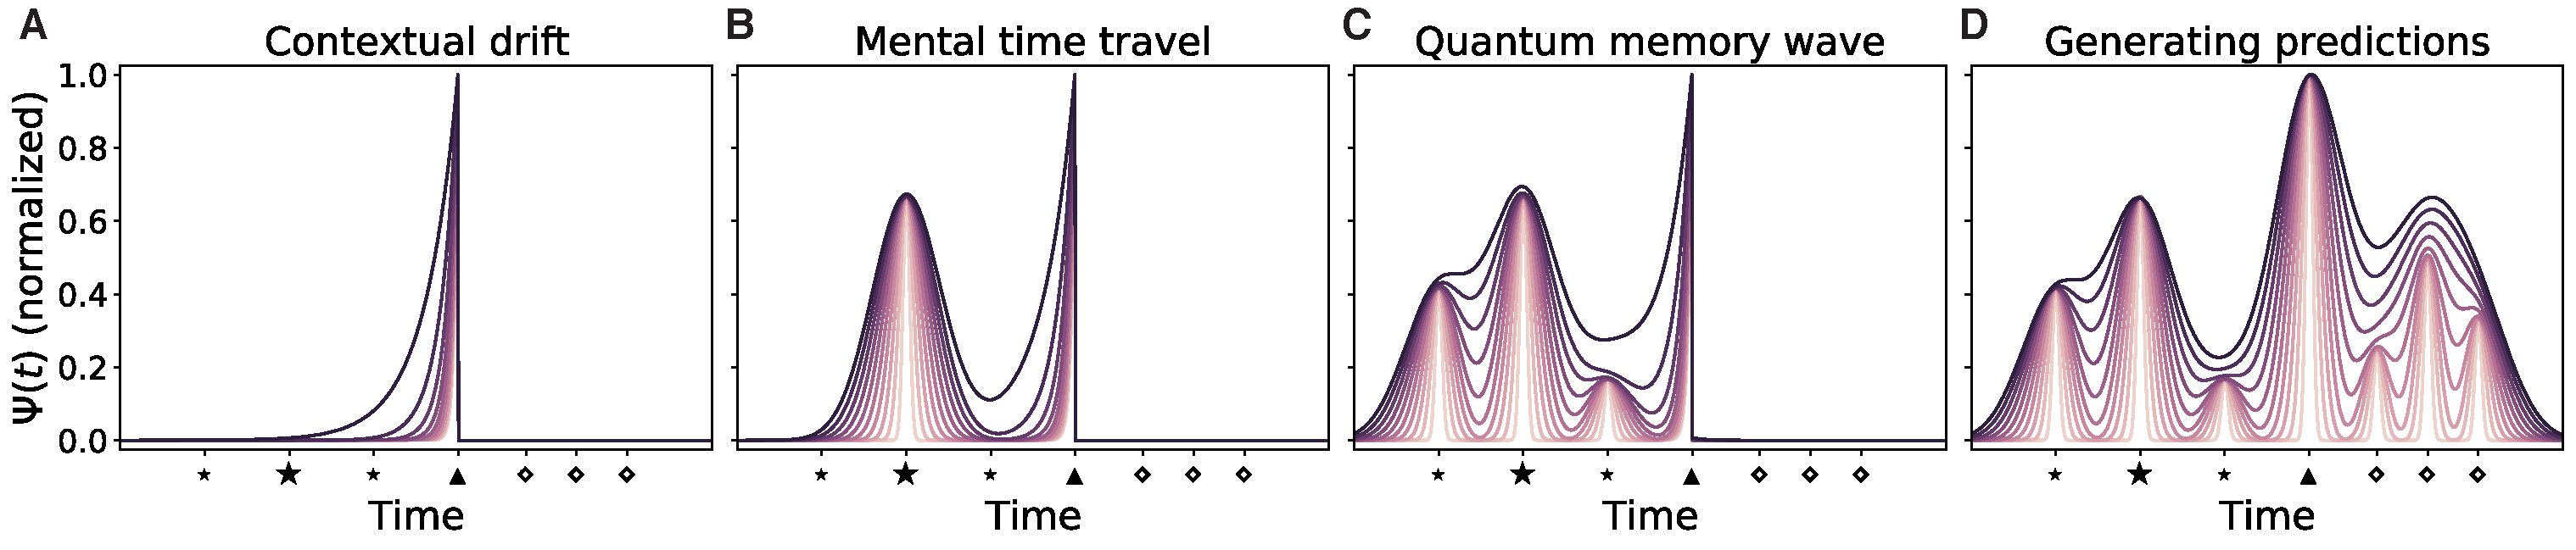
\includegraphics[width=\textwidth]{figs/wave_functions}
  \caption{\textbf{Memory wave functions. All panels.} Each panel displays a quantum memory wave function for a hypothetical individual at a particular moment (time $t=0$ indicated by $\blacktriangle$).  The $x$-axes correspond to the position ($t$) along the individual's autobiographical timeline.  The $y$-axes display how much the individual's thoughts at time $t = 0$ include information about the individual's past (or future) perceived or predicted experiences (i.e., at other times). Different colors denote different amounts of temporal blurring.  All curves have been normalized to have a maximum value of 1 and a minimum value of 0.  \textbf{A. Contextual drift (no explicit reinstatement).}  The blend of thoughts leading up to $t = 0$ reflects a recency-weighted average of information from the past.  \textbf{B. Mental time travel.} This constitutes a special case of the quantum memory wave function framework, whereby the individual's thoughts reflect a recency-weighted blend of prior thoughts, along with thoughts specific to one remembered prior experience (occurring at the timepoint indicated by the $\bigstar$ symbol).  \textbf{C. Quantum memory waves.}  In this example, the individual remembering the moment indicated by the $\bigstar$ symbol brings back a blend of thoughts similar to those shown in Panel B.  In addition, they bring to mind information pertaining to other conceptually related (but temporally non-contiguous) moments, indicated by $\star$ symbols. \textbf{D. Generating predictions about the future.} To predict what will happen during a series of future events ($\diamond$ symbols) the individual spreads their thoughts over their prior experiences according to the expected relevance of those experiences to the future events.  Local peaks in the curve denote prior experiences with high expected relevance.  The left part of the panel (prior to $\blacktriangle$) illustrates how the individual's thoughts are spread out over their past, and the right part of the panel illustrates how the individual's thoughts are spread out over their (predicted) future.}
\label{fig:qwave}
\end{figure}

The \textit{mental time travel} metaphor is defined by Tulving as ``the type of awareness experienced when one thinks back to a \textit{specific moment} in one's personal past and consciously recollects some prior episode or state as it was previously experienced''~\citep[Fig.~\ref{fig:qwave}B;][emphasis added]{WheeEtal97}.  Whereas mental time travel refers to mentally revisiting one specific moment in addition to now (potentially with some temporal blurring), the quantum memory wave framework implies that episodic memory entails spreading our awareness over \textit{many} moments (Fig.~\ref{fig:qwave}C).  In this way, the key distinction between these framings is whether remembering entails simultaneously revisiting one single moment versus many moments.  The two frameworks converge when we engage in \textit{chronesthesia}~\citep{Tulv02b}-- i.e., when we are consciously aware of subjective time.   Analogous to how measuring the physical location of a particle collapses its quantum wave function at the moment of measurement, engaging in chronesthesia can collapse our quantum memory wave function such that our thoughts temporarily converge on the moment we are revisiting.  This wave function expands again when our mental state changes in the next moment.

The quantum memory wave and mental time travel metaphors also diverge in explaining how we might predict what will happen in the future.  The quantum memory wave framing suggests that our predictions about the future draw from information pertaining to a blend of our prior experiences, weighted by their expected relevance to the future event in question (Fig.~\ref{fig:qwave}D).  To the extent that the mental time travel metaphor assumes that we can mentally visit just one other time (or time range) in addition to now~\citep[e.g.,][]{SzpuTulv11}, it is not clear how this sort of integration over temporally separated prior experiences might occur.  Specifically, integrating over those experiences would seem to require some mechanism for associating and simultaneously revisiting them while also casting some part of our thoughts forward to the future.

While the studies presented in the \textit{Introduction and overview} (on temporal receptive windows, the temporal window of integration, time cells, and temporal multiplexing) present strong empirical evidence that our brains maintain parallel representations at multiple timescales, questions remain about how or whether we experience those representations at a conscious level.  For example, are we consciously aware of spreading our mental states over many moments from our past?  Or is our subjective experience of remembering more like mentally time traveling back to a single ``hybrid'' moment that blends information from several of our (actual) prior experiences?

\section*{The temporal dynamics of ongoing experience and how we remember it}
Modern context-based theories of episodic memory posit that the current state of mental context serves to determine which information from our past may be relevant to us and therefore reactivated~\citep[e.g., ][]{PolyEtal09}. Although these theories were largely developed and tested in the domain of list-learning paradigms, conceptually similar principles might also underlie real-world memory.  For example, prior experiences with shared or overlapping contextual properties (e.g., other experiences that occurred in similar spatial or social settings, shared similar goals, etc.) could be leveraged to form schemas or situation models that help guide behaviors and expectations according to the current perceived context~\citep{RangRitc12, BaldEtal18, AlyEtal18}.

Unlike random word lists, naturalistic experiences contain \textit{event boundaries} whereby contextual cues change sharply from one moment to the next, implying a change in the current situation (e.g., shifting from the quiet peace of working on a manuscript in the early morning to the frenzied chaos of helping a newly awoken child get ready for school).  A number of studies (using non-random lists and more naturalistic stimuli) have found that the way we remember past experiences can be shaped by these event boundaries.  For example, controlling for elapsed time, memory is impaired for information that occurred prior to a change in the current event or situation~\citep[e.g., ][]{RadvCope06, SwalEtal09, SwalEtal11, EzzyDava11, MannEtal16}.  The temporal dynamics of contextual change also underlie how we judge the amount of time elapsed since a prior reference point~\citep{BlocReed78, SahaSmit14}.  These findings suggest that the rapid contextual or situational changes that define these event boundaries shape how we experience and remember~\citep{DuBrDava16}, similarly to how spatial boundaries~\citep[e.g., environmental barriers;][]{McKeBuzs16, BrunEtal18} shape how we experience and remember spatial environments and layouts, or how conceptual boundaries~\citep[e.g., distinctions between semantic categories;][]{BrunEtal18} shape how we experience and remember conceptual information.

Event boundaries are one example of the broader temporal covariance structure that is characteristic of ongoing experience.  Whereas classic approaches to studying memory (e.g., list-learning paradigms and other trial-based experiments) encourage researchers to treat each moment, trial, or stimulus as separable from the rest of experience, context-based theories of memory (including situation models and event-based models) posit that each moment derives meaning through its deep ties to other related (but potentially temporally separated) experiences.  This rich tapestry of interacting moments and experiences forms a scaffolding for interpreting our new experiences and for retrieving information concerning our past.  According to this view, the reactivation of this rich tapestry of contextual details enfolding the remembered event (i.e., how the event relates to the rest of one's experiences across timescales) is even more central to our subjective experience than the specific details of what occurred during that event!  This begs the question: which thoughts, from which times, do we reactivate when we remember our past experiences?

\subsection*{How is our past replayed when we remember?}
Our ongoing experiences can cue us to remember information about our past.  This can happen explicitly (e.g., during a conversation about a specific prior event) or implicitly (e.g., when something happening now reminds you of what happened before).  Context-based theories of memory posit that the particular memories that our ongoing experiences cue will be related~\citep[contextually, semantically, functionally, etc.; e.g., ][]{PolyEtal09}.  One potential challenge to studying how we remember the past relates to detangling which links between our experiences are specifically driven by our memory systems versus which are imposed ``externally'' through the similarity structure of those experiences.  For example, consider your daily commute into work.  If you were to verbally recount a specific day's commute later, one might expect some aspects of your description to apply to other days' commutes as well (e.g., other commutes where you took a similar route or travelled via similar modes of transportation, listened to similar music along the way, travelled at a similar time, etc.).  But to what extent could one hope to separate out descriptive matches driven solely by similarities in those commuting experiences, versus true reactivations (in memory) of specific memories of those other prior commutes?

One insight into this distinction comes from a recent study by \cite{HeusEtal18c}, which analyzed data collected by \cite{ChenEtal17} who had participants watch an episode of the BBC television show \textit{Sherlock} and then verbally recount what happened in the episode.  The authors used topic models~\citep{BleiEtal03} applied to human-generated annotations of each camera shot in the episode to characterize the episode's content with a timeseries of high-dimensional semantic feature vectors (see \textit{Defining the geometries of ongoing thoughts and memories}).  Each shot's annotation contained the following information: a brief narrative description of what was happening, the location where the scene took place, whether that location was indoors or outdoors, the names of all on-screen characters, the names of the character(s) who were in focus in the camera shot, the name(s) of any character(s) who spoke during the scene, the camera angle of the shot, a transcription of any on-screen text, and whether or not there was any music present in the auditory background~\citep[full details may be found in][]{ChenEtal17}.  The resulting \textit{topic vectors} describe the mix of ``themes'' present in each moment of the episode (Fig.~\ref{fig:embedding-models}B).  When characterized in this way, the episode's content exhibits periods of relative stability, followed by moments of rapid change. This interplay between stability and change is visible as ``blocks'' in the temporal correlation matrix (Fig.~\ref{fig:corrmats}A); \cite{HeusEtal18c} performed detailed analyses of these putative \textit{events} and how they are remembered.  Notably, the off-diagonal entries of the temporal correlation matrix (which reflect content similarity between temporally distant events in the episode) are nearly all close to 0.  This is surprising, because the episode itself comprises a murder mystery with recurring motifs that must be associated in the viewer's mind in order to make sense of the episode.  Nonetheless, when considering solely the semantic content of each moment of the episode, those long timescale associations are nearly entirely absent.  To the extent that this finding extends to real-world experiences, it comports with Heraclitus' notion that one cannot step in the same river twice~\citep{Hera}.

\begin{figure}[tp] \centering 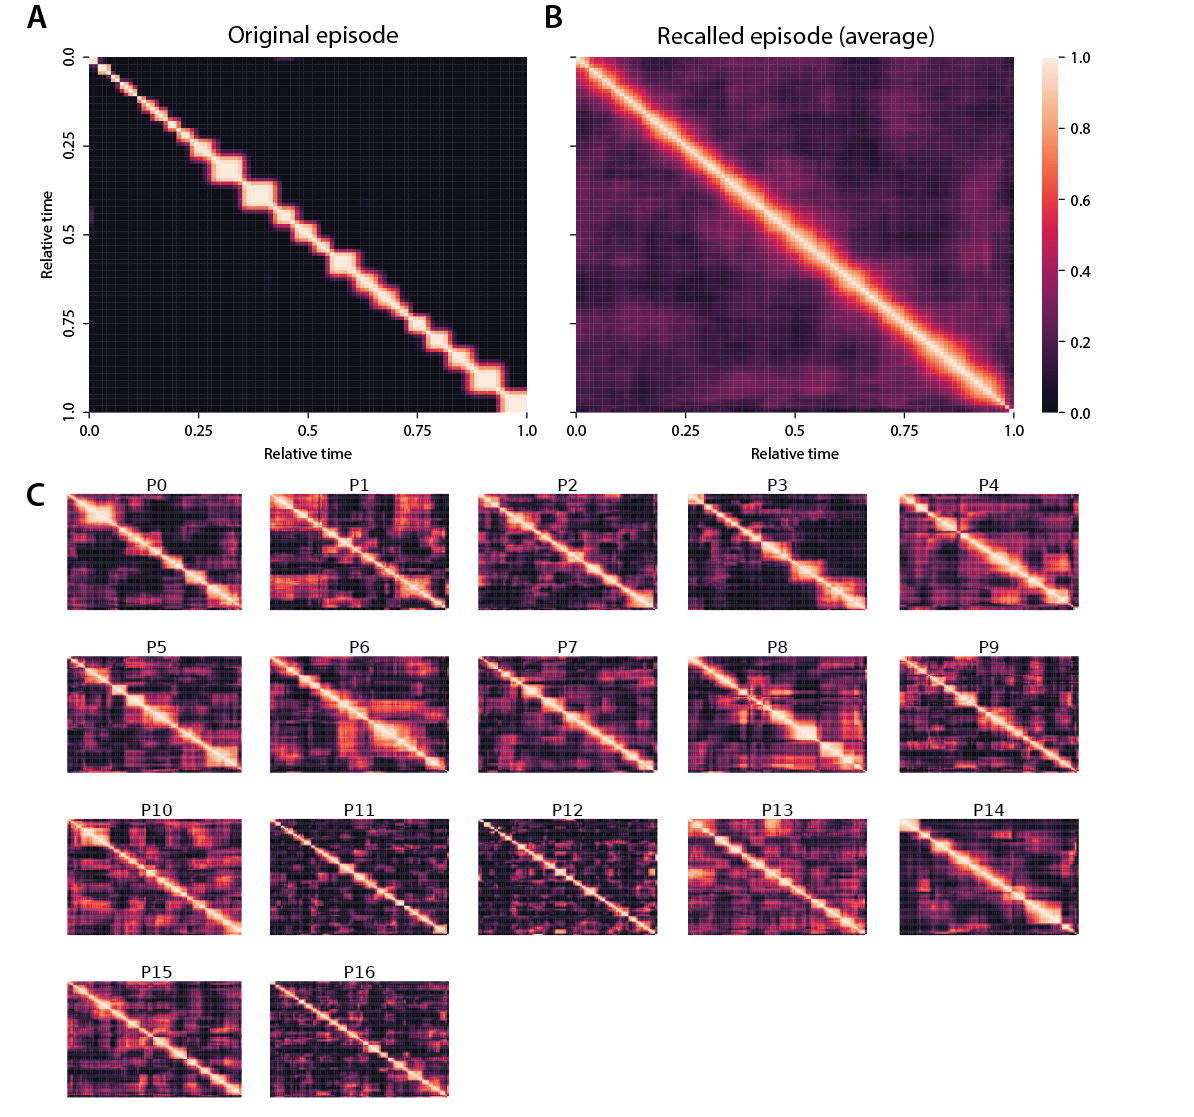
\includegraphics[width=0.8\textwidth]{figs/pres_rec_corrmats_sherlock} \caption{\textbf{Temporal correlation matrices of the dynamic content of a television episode and people's recalls of that episode.}  The panels of this figure are adapted from \cite{HeusEtal18c}, where full details may be found. \textbf{A. Temporal correlations exhibited by the content of the television episode.}  Each moment of an episode of the BBC television show \textit{Sherlock} has been characterized using a topic model~\citep{BleiEtal03} fit to detailed human-generated annotations between each scene cut.  The correlations between the topic vectors of a given pair of timepoints reflects the similarity in thematic content at those timepoints.  \textbf{B. Temporal correlations exhibited by the (average) content of participants' recalls of the episode.} The topic model used to characterize the episode in Panel A has been applied to each sentence from each participants' recall transcript.  The temporal correlation matrices describing each participants' recalls were re-sampled using cubic interpolation to have 100 rows and columns prior to averaging the resampled matrices across participants.  \textbf{C. Temporal correlations in the content of individual participants' recalls of the episode.} Each sub-panel displays the temporal correlation matrix for one experimental participant.}
\label{fig:corrmats}
\end{figure}

Although the specific mix of contents in each moment of the episode is nearly unique, participants' subjective experiences of the episode entail weaving together those temporally separated moments into a cohesive narrative.  This is reflected in how people verbally recount the episode later.  If we examine the temporal autocorrelation matrices of participants' recalls of the television episode (characterized using the same topic model used to capture the content of the episode; Figs.~\ref{fig:corrmats}B, C), we see a different structure than that of the episode itself.  Although individual participants' recalls also exhibit periods of content stability punctuated by rapid change (visible in the blocky structure of the matrices in Fig.~\ref{fig:corrmats}C), the off-diagonal correlations between the thematic content of temporally distant events are substantially stronger in participants' recalls than in the original episode.  Another way of characterizing this phenomenon is to look at the autocorrelation functions (describing the correlation between different moments' topic vectors as a function of their temporal distance) for the episode versus participants' recalls (Fig.~\ref{fig:reinstatement}A).  Whereas the autocorrelations in the original episode's content rapidly fall to 0, autocorrelations in the content of participants' recalls appear to asymptote around an average of 0.2.  These analyses indicate that the way participants \textit{recount} temporally separated events imposes additional similarity on those events, beyond what was present in the original events themselves.  One can then ask: is this simply a matter of imprecision in recall, either with respect to participants' recalls themselves, or with respect to the quality with which they are characterized via semantic feature vectors?  Or might there be a functional role of that additional imposed similarity structure?

To understand which specific events are described (during recall) as more similar than what their original experiences (as characterized by their topic vectors) would suggest, it can be helpful to examine individual recalls of particular events throughout the episode.  Figure~\ref{fig:reinstatement}B displays, for a representative example recalled event, which other parts of the episode were characterized in a similar way by the participants when they recounted the episode later (black and colored lines), and which other parts of the episode were described in a similar way in moment-by-moment (non-recall) human annotations (gray line).  In the example event explored in the figure, Sherlock Holmes and John Watson (main characters) are bantering, and then are interrupted when Sherlock realizes that another person has committed suicide.  Later the viewer learns that the suicides were actually murders.  The language used by human annotators describing the moment-by-moment contents of the event used a similar mix of themes only for temporally nearby parts of the episode (gray line).  However, the way participants described what happened when they \textit{recounted} the episode later revealed a much different pattern.  Specifically, their language mirrored that used when they were recalling other related murders, and other moments when Sherlock and John were bantering with or about each other (Fig.~\ref{fig:reinstatement}C).

The way they described the example target event did \textit{not} mirror the way they described other events that were not directly narratively linked with the target event, even when those other events overlapped semantically.  For example, thematic elements of events involving unrelated violence, or Sherlock and John interacting with other characters about other subjects, tended not to feature in participants' recountings of the target event.  Taken together, this suggests that these specific events were associated in participants' memories, perhaps contributing to (or reflecting) their understanding that those events were linked in the episode's narrative.

One concrete example of this phenomenon is that early in the episode, including during the target event, Sherlock and John appear to be investigating a series of suicides.  Later in the episode, it becomes clear that the apparent suicides are actually murders.  The annotations refer to early deaths (including that shown in Fig.~\ref{fig:reinstatement}B) as suicides, whereas participants often refer to those early deaths as ``murders'' even though they could not have known that they were murders early on in the episode.  In this way, participants' experiences \textit{subsequent to} a target remembered event may distort its memory by incorporating information learned during other experiences.

\begin{figure}[tp] \centering 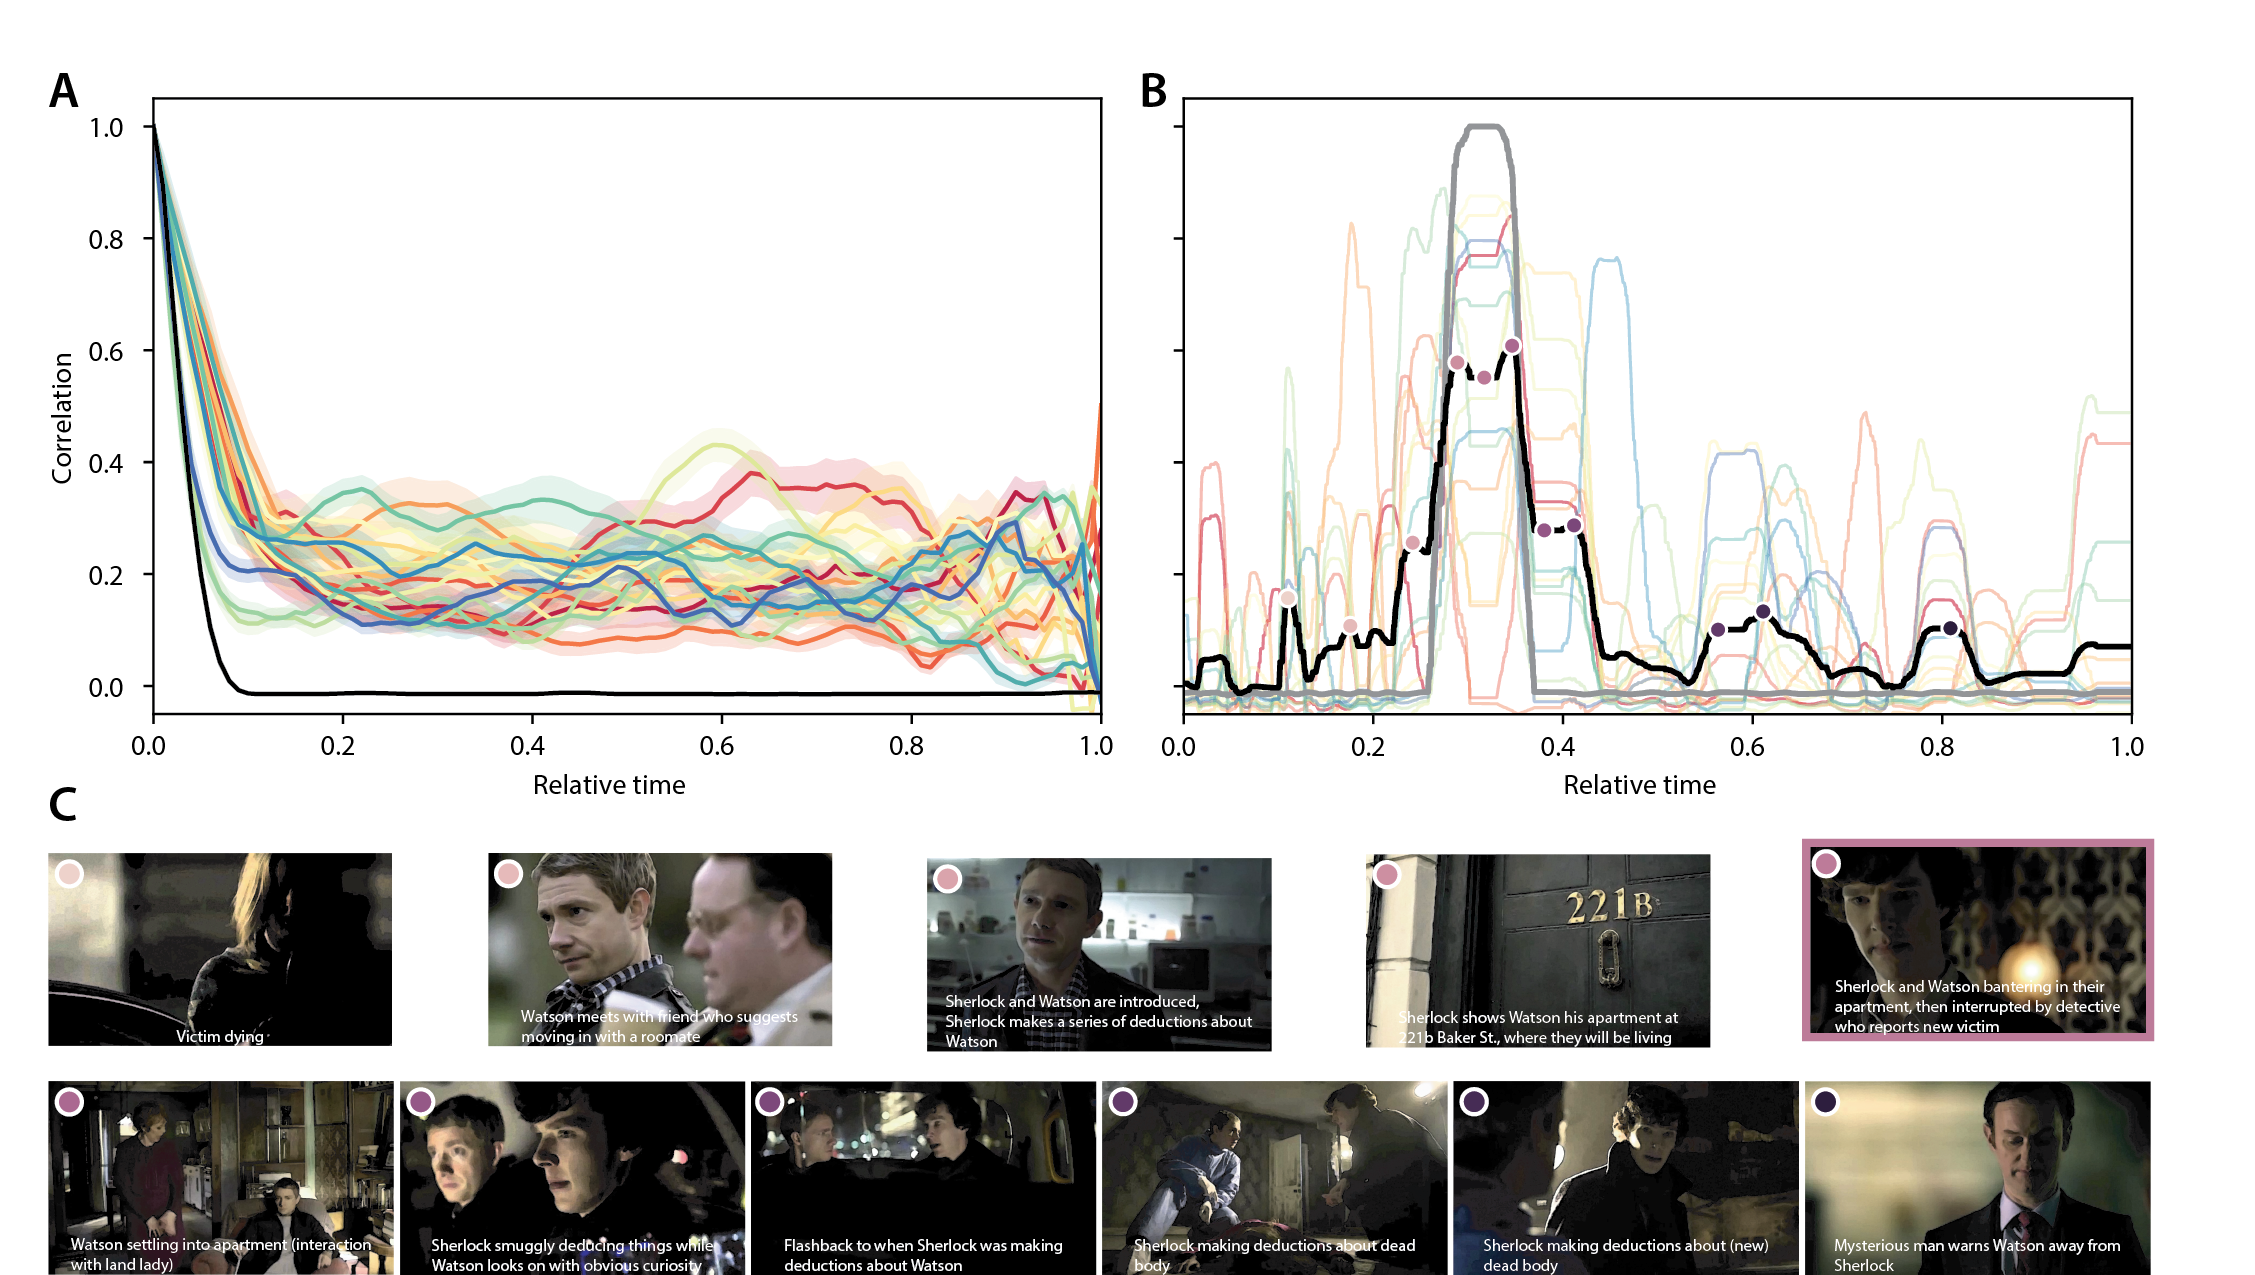
\includegraphics[width=\textwidth]{figs/reinstatement} \caption{\textbf{Content drift in a television episode and participants' recalls of that episode.  A.  Autocorrelations in the episode's content and in the content of participants' recalls.}  The black line denotes the average correlations between the topic vectors from pairs of moments in the episode as a function of their temporal separation (times are relative to the full length of the episode).  Each colored line denotes an analogous autocorrelation function, but for each individual participant's recalls of the episode (times are relative to the full length of each participant's recalls).  The error ribbons denote 95\% confidence intervals, taken across all moments in the episode (or in participants' recalls of the episode).  \textbf{B. Recall density functions for one recalled event.} Each curve reflects the correlations between the topic vector at each (relative) moment of the episode (or participants' recalls of the episode), and the topic vector of an event beginning approximately $\frac{1}{3}$ through the episode (relative time: 0.328).  The gray curve denotes these correlations for the topic vectors derived from annotations of the episode itself. The black line denotes the average correlations across all participants' recalls.  Local maxima are marked with colored dots.  Local maxima closer than 2.5\% of the total recall duration to a higher local maximum were excluded (this constraint served to eliminate very nearby peaks that corresponded to duplicate events), as were maxima with peaks with correlation coefficients lower than 0.1 (this threshold was chosen arbitrarily; this constraint served to eliminate events that were only very weakly associated with the example event).   The colored lines denote the correlations for each individual participant's recalls.  \textbf{C. Local maxima in the average recall density function.}  Representative screen captures from the scenes at each local maxima in Panel B are displayed (dot colors match those in Panel B).  The text in each screen capture displays a brief summary of what happened in each scene. The colored outline denotes the reference scene being recalled.}
  % colors: individual participants
  % black: average across participants
  % gray: autocorrelation with topic vector at timepoint
  % circles: local maxima in the across-participants average (i.e., movie events that share structure with the given timepoint that is distinct from other temporally proximal events)
\label{fig:reinstatement}
\end{figure}

A recall density function analogous to the one displayed in Figure~\ref{fig:reinstatement}B could, in principle, be characteristic of memory for \textit{any} past event or experience.  For example, the peaks of the function could provide insight into which events, from which moments along one's autobiographical timeline, are functionally associated in memory.  Nonetheless, a potential challenge to testing this hypothesis in the laboratory is that in many memory studies there is no particular reason for participants to functionally associate the stimuli.  For example, there is often no ``deeper narrative'' to make sense of in list-learning studies or in most standard trial-based memory experiments.  However, random word list learning experiments might happen to contain (for a given list) semantically related words.  Indeed, a number of studies indicate that participants spontaneously form associations between semantically related words on random word lists, even when those related words are separated in time~\citep[e.g.,][]{WixtRohr94, MannKaha12, MannEtal12}.  This suggests that our memory systems pick up on statistical regularities, even in ostensibly ``random'' stimulus sequences, and that we leverage those regularities when we recall our past~\citep{PolyEtal09}.  Other work suggests that our memory systems may also leverage these regularities to parse our ongoing experiences into discrete events~\citep{SchaEtal13, Shap19}.  Are these examples in the literature on random list learning studies, indicating that our memory systems leverage ``accidental'' structure in random sequences, a reflection of the same fundamental principle driving the memory reactivation function displayed in Figure~\ref{fig:reinstatement}B?

It is difficult to explicitly test whether (apparent) semantic reinstatement in word list learning, as reflected in people's tendencies to semantically cluster recalls of random word lists, reflects integration of information across the experiences of studying those words.  However, remembering word lists does not specifically \textit{require} integrating information across words in order to gain a deep understanding of the list.  By design, there \textit{is} no deeper meaning of random word lists.  One way to characterize the meaning reflected by how an experience unfolds in time is through models that describe the geometric path that the experience takes through an appropriate representational space.


\section*{The shapes of remembered experiences}
The study by \cite{HeusEtal18c} described above suggests one way of characterizing the dynamic content of complex naturalistic stimuli like television episodes.  The sequence of topic vectors over the course of the episode traces out a \textit{topic trajectory} through a high-dimensional feature space.  The sequence of topic vectors for a given participant's recalls traces out an analogous trajectory.  This characterization provides a geometric framework for comparing the \textit{shapes} that reflect how naturalistic experiences unfold over time, to the shapes of how we remember those experiences later (Fig.~\ref{fig:trajectories}).  One can then use the geometric transformations needed to map an experience's trajectory onto the trajectory of its later remembering to characterize the quality and content of memory.

\begin{figure}[tp]
\centering
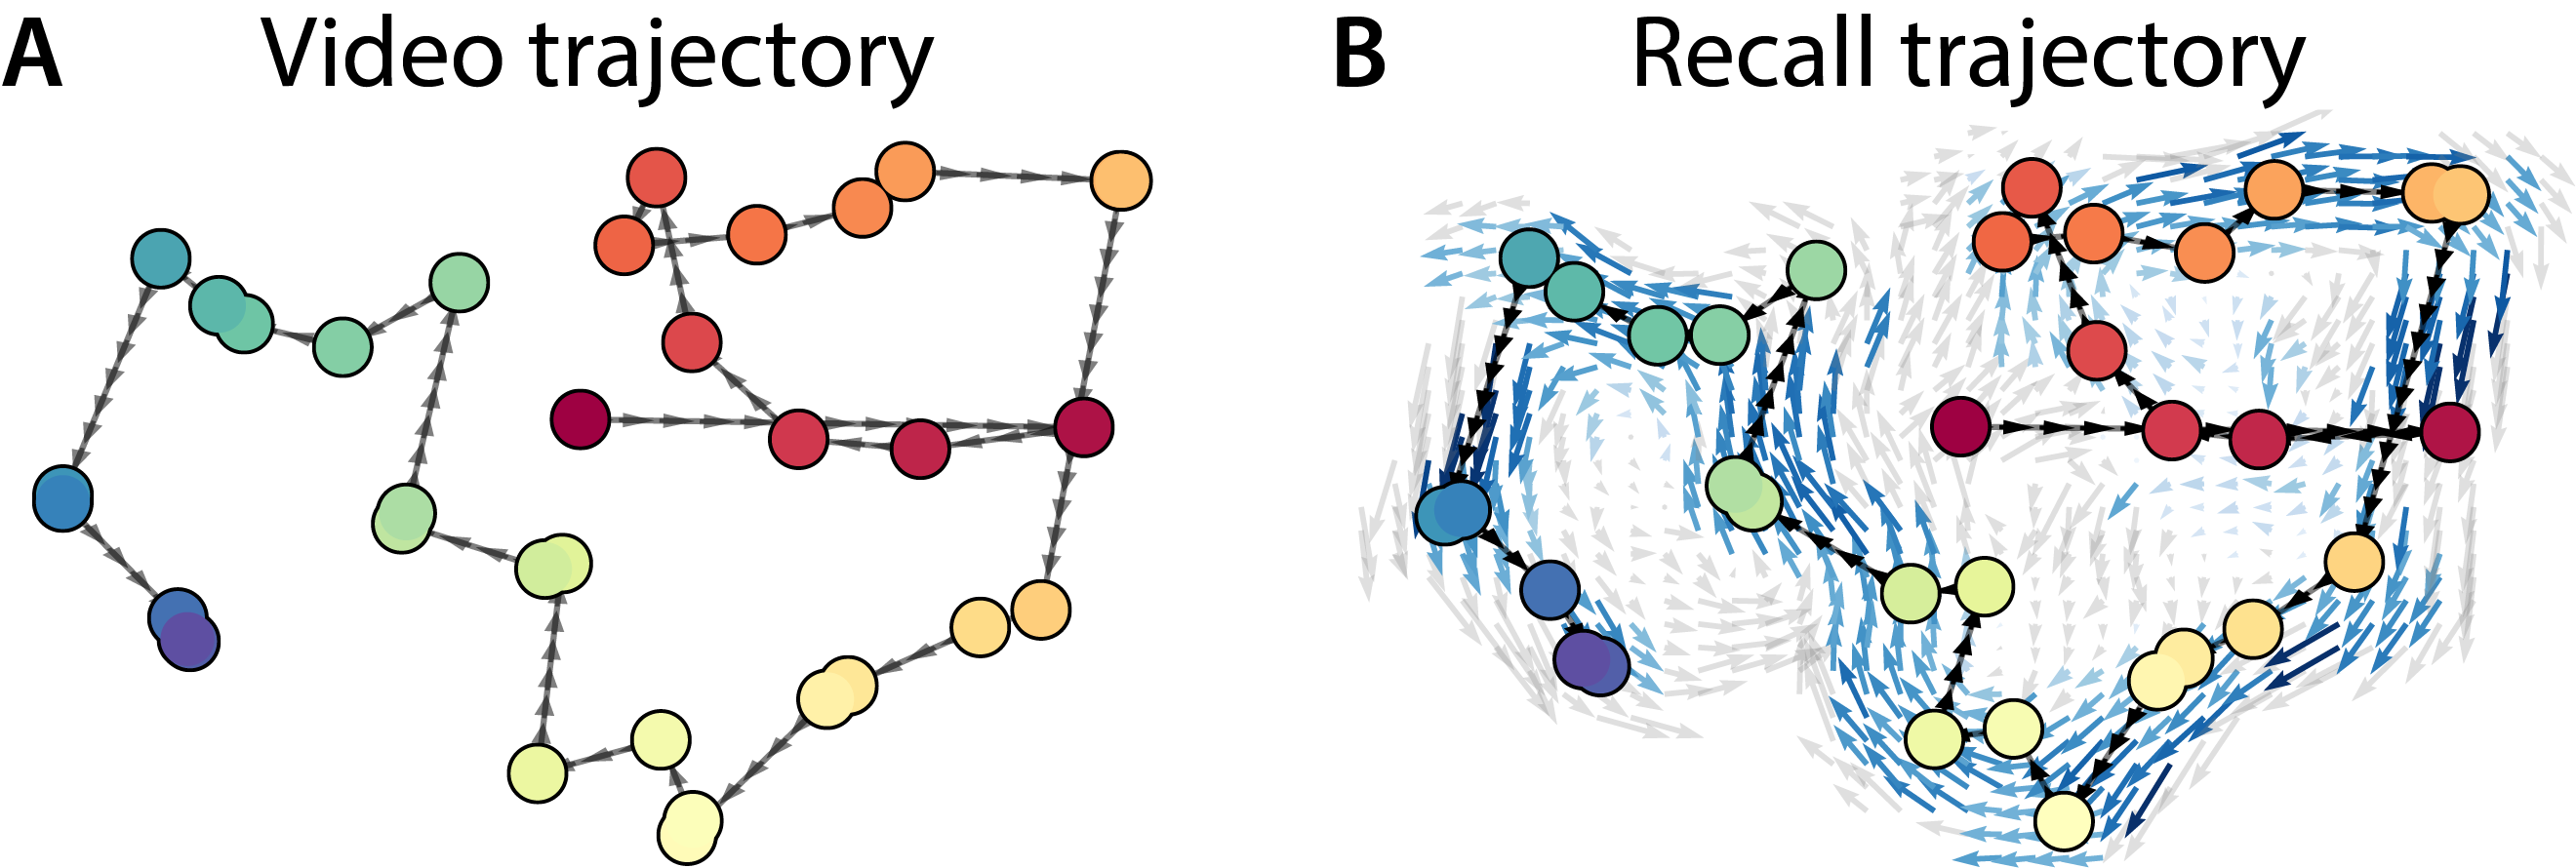
\includegraphics[width=0.8\textwidth]{figs/trajectory}
\caption{\textbf{The shape of an unfolding experience.}  \textbf{A. The trajectory through topic space taken by a television episode.} The topic trajectory taken by a 50 minute television episode, projected onto two dimensions.  Each dot indicates an event identified using a Hidden Markov Model; the dot colors denote the order of the events (early events are in red; later events are in blue), and the connecting lines indicate the transitions between successive events.  \textbf{B. The trajectory through topic space taken by participants' recalls of the television episode.} The average two-dimensional trajectory captured by 17 participants' recalls of the episode, with the same format and coloring as the trajectory in Panel A. The arrows reflect the directions of the average transitions taken by participants whose trajectories crossed that part of topic space; blue arrows denote directions of reliable agreement across participants.  Figure adapted from \cite{HeusEtal18c}, where additional details may be found.}
\label{fig:trajectories}
\end{figure}

In addition to serving as a framework for quantifying the dynamic content of experiences, these trajectories may be visualized by projecting word embedding representations of the events onto lower dimensional spaces~\citep[e.g., ][]{HeusEtal18a}; for additional discussion and counterpoints see~\cite{JollChan18}.  \cite{HeusEtal18c} applied this approach to the same dataset reflected in Figures~\ref{fig:corrmats} and~\ref{fig:reinstatement}, revealing another key property of how we remember.  Although there are substantial individual differences in the specific words people use to describe their shared experience of watching the same television episode, and how much detail they recollected, the overall shapes of those recalled experience trajectories are highly similar across people.  This has potentially exciting implications for what it means to communicate memories to other people: to effectively communicate, we often need to convey the ``essence'' (gross overall shape) of our experience.  It also has implications for how we learn by analogy: perhaps events that share schemas~\citep[e.g., ][]{BaldEtal18}  unfold in similar ways (e.g., have similar shapes).  Learning which shapes go with which schemas could provide a scaffolding for rapid learning and generalization of new experiences, to the extent that those new experiences match a previously learned schema (shape).

In their paper, \cite{HeusEtal18c} use the geometric shapes of experience trajectories (through word embedding space) to functionally distinguish high-level essential details of the experience from low-level (non-essential) details.  When the trajectory exhibits a sharp change in direction, this indicates a rapid shift in the thematic content of the episode.  \cite{HeusEtal18c} used hidden Markov models to detect these rapid shifts and segment the trajectories into discrete \textit{events}.  The high-level (essential) details of the episode are reflected in the shape defined by the sequence of coordinates of its events.  These are captured by low spatial frequency properties of the trajectory's shape.  Low-level details are characterized by (typically smaller-scale) within-event geometric patterns, which are captured by the high spatial frequency properties of the trajectory's shape.  A key finding of that work was that people who watched the episode recalled high-level details reliably, and in a similar way across people, whereas people varied substantially in how they remembered low-level details.  This suggests that our memory systems may prioritize certain types of information (e.g., high-level details) about our experiences over others (e.g., low-level details) as we encode our experiences into memories or when we recount our prior experiences.

\subsection*{The \textit{matching problem}}
The trajectories through word embedding space displayed in Figure~\ref{fig:trajectories} demonstrate that topic models are sufficiently expressive and robust to provide one solution to the \textit{matching problem} in memory analysis.  The matching problem refers to discovering an alignment in the labels between experienced and remembered events.  Traditional memory paradigms most commonly studied over the past century~\citep{Kaha12} ask participants to study lists of \textit{items} (often randomly selected words) and then engage in a memory task, such as verbally recalling any words the participant remembers studying, in any order.  Solving the matching problem in such experiments is trivial: if we treat each studied word on a list as an ``event,'' then we can assume that the participant is remembering a word's event when they verbalize that word during their memory test.  In other words, matching entails finding the exact match between a word the participant is verbalizing and that same word on the list that they studied.

For real-world memory phenomena, and in many naturalistic memory paradigms, solving the matching problem is more complex.  People often experience real-world events (and scenes from movies or stories) as rich sensory experiences that derive deep meaning from surrounding moments, other prior experiences, emotions, goals, high-order understanding of the current situation, and so on.  Many of these aspects of our real-world experiences are not immediately verbalizable-- and even when we are able to describe some specific aspects of what we are experiencing, there are typically many possible ways we could have done so (e.g., varying in level of detail, specific wording, objectivity versus subjectivity, contextual details, etc.).  Further, because the way we experience each moment depends in part on our unique prior experiences, even ostensibly shared experiences can \textit{seem} different to each individual.  The way we recount a given experience is often a reflection of our own idiosyncratic experience of the original event, and is colored and distorted in an idiosyncratic way by our memory systems.  This distorted memory must then be verbalized or communicated, which is itself an idiosyncratic (and potentially lossy, in the information theoretic sense) process.  Solving the matching problem under these constraints poses a substantial theoretical and methodological challenge.  Specifically, matching requires building explicit models of the dynamic conceptual content of our experiences and memories, and then estimating when and how that experienced and remembered content aligns.  The approach featured in Figure~\ref{fig:trajectories} uses a word embedding space that is defined by a topic model~\citep{BleiEtal03}.  Each coordinate in this space reflects the conceptual content underlying a set of words, such that two different text passages that describe the same conceptual content (but using different words, levels of detail, etc.) are mapped onto nearby points in the word embedding space.  When these models are sufficiently expressive and robust to solve the matching problem, by modeling our experiences and memories within the same word embedding space, we can see a clear geometric alignment between the trajectories that our experiences (Fig.~\ref{fig:trajectories}A) and memories (Fig.~\ref{fig:trajectories}B) take through word embedding space~\citep[also see][]{HeusEtal18c}.

\subsection*{Defining the geometries of ongoing thoughts and memories}
Defining geometric spaces that can reliably capture the conceptual contents of our thoughts and experiences has become a major focus of computational science.  One family of models that has shown particular promise over the past several decades is broadly referred to as \textit{word embedding models} (Fig.~\ref{fig:embedding-models}).  The fundamental goal of these models is to take as input a sequence of words (text) and produce as output one or more feature vectors whose coordinates reflect their conceptual (semantic) content.  For example, when two conceptually similar documents are passed through these models, the goal is to produce two feature vectors that are closer (e.g., in Euclidean distance) than the feature vectors for two dissimilar documents.

Early word embedding models such as \textit{Latent Semantic Analysis}~\citep[LSA;][]{DeerEtal90, LandDuma97} derived text embeddings using word co-occurence statistics.  The logic driving this approach posits that documents that contain similar mixtures of words are likely to be conceptually similar, and words that appear in similar documents are also likely to be conceptually similar.  To quantify these intuitions, \cite{DeerEtal90} first constructed \textit{word count matrices} (Fig.~\ref{fig:embedding-models}A) for several text corpora (each comprising many thousands of documents).  Each entry in these matrices denotes the number of times a given document (row) contained a given word (column).  They then used the Singular Value Decomposition (SVD) to decompose the number-of-documents $~\times~$ number-of-words word count matrix into the product of a number-of-documents $\times~K$ \textit{document embeddings matrix}, a $K~\times~K$ \textit{singular values matrix}, and a $K~\times$ number-of-unique-words \textit{word embeddings matrix}.  The rows of the document embeddings matrix reflect the similarities between documents, and the columns of the word embeddings matrix reflect similarities between words.

A related approach, termed \textit{Word Association Spaces}~\citep[WAS;][]{NelsEtal04, SteyEtal04} replaces the word count matrix with data from a large free-association experiment.  In the experiment, each participant was asked to free-associate (i.e., say the first word that came to mind) in response to a series of cue words.  The authors then constructed a number-of-cue-words $~\times~$ number-of-unique-response-words matrix whose entries reflected the proportion of times each cue word (row) produced a given response word (column) across participants.  After using SVD to decompose this \textit{word frequency matrix}, they obtained low-dimensional embeddings of each cue word and response word.  In one sense, WAS might provide a more accurate and behaviorally relevant reflection of how people think about the meanings of words than LSA, since nearby WAS vectors reflect either cue words that produced similar responses, or response words that were evoked by similar cues.  In other words, WAS derives embeddings directly from people's semantic judgement behaviors.  However, because WAS is based on a large amount of experimental data, updating the embeddings requires collecting new data, which can be slow and costly.  As the target application or population diverges from the experimental population (e.g., over time, across cultures, demographics, etc.) the WAS embeddings may become less accurate or relevant.  By contrast, LSA may be re-fit relatively quickly to any new corpus, enabling the resulting embeddings to stay current.  Further, because LSA may be applied to any corpus, word embeddings may be easily computed and/or compared across languages, times, subject areas, etc.

\begin{figure}[tp]
\centering
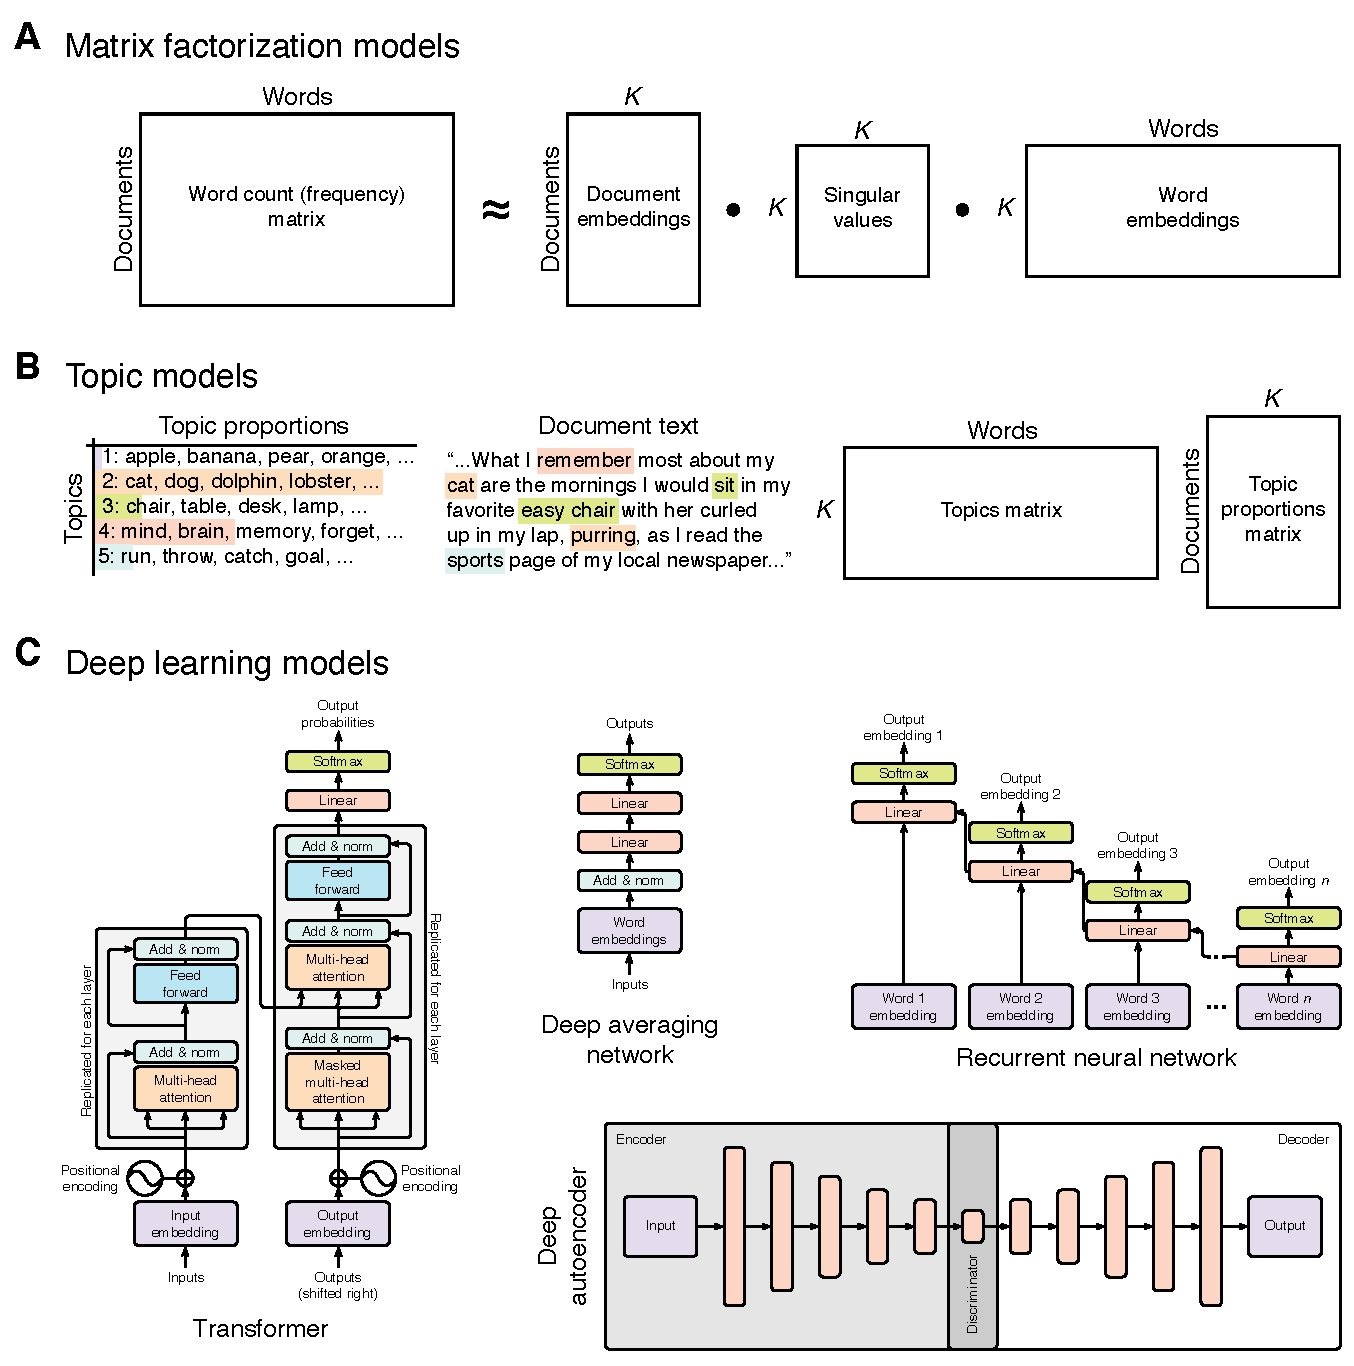
\includegraphics[width=0.8\textwidth]{figs/word_embedding_models}
\caption{\textbf{Three approaches to text embedding.}  \textbf{A.~Matrix factorization models.} Per-document (or per-stimulus) word counts and/or frequencies are collected into a word count matrix (left).  To compute $K$-dimensional embeddings of the documents and words, the word count matrix is factorized (typically by computing its Singular Value Decomposition) into the product of a number-of-documents $\times~K$ \textit{document embeddings matrix}, a $K \times K$ \textit{singular values matrix}, and a $K~\times $ number-of-unique-words \textit{word embeddings matrix}.  \textbf{B.~Topic models.}  Fitting a topic model to a word count matrix (e.g., Panel A) reveals a set of latent \textit{topics}, or themes that pervade each document.  The topics are specified in a $K~\times$ number-of-words \textit{topics matrix}, and the per-document themes are specified in a number-of-documents $\times~K$ \textit{topic proportions matrix}. A given document's topic proportions reflect the specific mix of themes that are reflected in that document (bar graph on the left).  These proportions are discovered automatically by estimating the topic from which each word in the document is most probably drawn (highlighted words in \textit{Document text}).  \textbf{C.~Deep learning models.}  A wide variety of deep learning approaches to text embedding have been proposed.  Broadly, these approaches often combine a common set of elements, including \textit{transformers}~\citep[diagram adapted from][]{ViswEtal17}, \textit{deep averaging networks}~\citep[diagram adapted from][]{IyyeEtal15}, \textit{recurrent neural networks}~\citep[diagram adapted from][]{IyyeEtal15}, and \textit{deep autoencoders}~\citep[diagram adapted from][]{YousHame17}.}
\label{fig:embedding-models}
\end{figure}

\textit{Topic models}, such as \textit{Latent Dirichlet Allocation}~\citep[LDA;][]{BleiEtal03} represent an attempt to characterize the latent \textit{topics} or themes that documents comprise (Fig.~\ref{fig:embedding-models}B).  Whereas matrix factorization approaches represent semantic meanings using low-dimensional approximations of word co-occurrences or free association frequencies, topic models leverage these properties of documents (or behaviors) to explain \textit{why} words co-occur.  LDA defines a topic as a distribution of weights over words in the vocabulary.  For example, if one takes the \textit{vocabulary} to be the top 10,000 most commonly used words in English (excluding stop words that are devoid of explicit semantic meaning such as ``and,'' ``or,'' ``the,'' ``but,'' etc.), then each topic comprises a vector of 10,000 non-negative weights that sum to one.  As shown in the cartoon on the left of the Panel (where the four top-weighted words from each of five hypothetical topics are displayed), a fruit-related topic (shown in purple) might weight heavily on words like ``apple,'' ``banana,'' ``pear,'' and ``orange,'' whereas words like ``cat,'' ``dog,'' ``dolphin,'' and ``lobster'' might receive relatively small weights.  Given a set of $K$ topic vectors, topic models compute the blend of topics most probably reflected in a given document-- i.e., its \textit{topic proportions}.  These topic proportion estimates are made by examining how different topics weight each of the words in the document, and by assuming that documents tend to reflect few topics (rather than many topics).  Given only a word count matrix as input (just as in LSA), topic models automatically discover a $K~\times~$ number-of-words \textit{topics matrix}, which describes how each topic (row) weights each word in the vocabulary (column), and a number-of-documents $~\times~K$ \textit{topic proportions matrix}, which describes each document's topic proportions.  The rows of the topic proportions matrix may be treated as low-dimensional embeddings of the set of documents.

A key advantage of topic models over matrix factorization models is their ability to explain potentially ambiguous word usage.  For example, consider the use of the word ``bat'' in the following illustrative passage:
\begin{quote}
  \textit{``As the slavering mutant vampire \textbf{bat} swooped low to attack, its eyes ablaze, the explorer grunted and took a mighty swing of her trusty aluminum baseball \textbf{bat}.  The powerful strike connected with an echoing metallic \textit{clink}, stunning the wretched creature before it scrambled about on the cave floor and flew away.  She didn't even \textbf{bat} an eye-- as the Dark Wizard Chiroptera continued to draw strength from the mystic crystals, such things had become increasingly common of late, nearly to the point of mundanity...''}
  \end{quote}
At different ponts in the passage, ``bat'' refers to an animal, a piece of sports equipment, and an eye-related verb.  Because each of these uses of the word appears in the same (hypothetical) document, models driven solely by word co-occurrence statistics would blend these different meanings such that the embedding of ``bat'' was somewhat similar to other animals \textit{and} other pieces of sports equipment \textit{and} other eye-related verbs.  By contrast, treating each document as reflecting a blend of topics allows these uses to be disambiguated.  If other documents that mention the word ``bat'' describe vampires, swooping, or other mammals, but \textit{not} sports equipment or eye-related verbs, then a topic model could explain this pattern by inferring that multiple topics place substantial weight on the word ``bat.''  Another strength of topic models is their interpretability.  Because the models directly output each document's topic proportions along with each topic's weights on all words in the vocabulary, the general themes that each topic reflects are often intuitive and the per-document topic proportions may be directly related to those themes.

Both the matrix factorization models and topic model described above are each examples of \textit{bag of words} models.  Given a document, these models will generate the same embeddings for any random re-ordering of the same words.  This over-simplifies the intended conceptual content of documents, where word order often conveys important meaning.  An alternative framing of the text embedding problem is to use \textit{sequence} models that explicitly account for word order effects.  Most modern sequence-based models are implemented using deep neural networks (Fig.~\ref{fig:embedding-models}C).

The \textit{Neural Probabilistic Language Model}~\citep[NPLM;][]{BengEtal03} was one of the earliest deep learning-based sequence models.  NLPM derives word embeddings for each word in the vocabulary (such that nearby embeddings reflect semantically related words), and then models word sequences according to their meanings.  This model was inspired in part by $n$-gram models~\citep{BrowEtal92}, which estimate the probability of the next word in a sequence given the $n$ words that came before it. Effectively, NLPM attempts to learn arbitrarily long sequences.  In a related approach, \cite{MnihHint09} proposed the \textit{Scalable Hierarchical Distributed Language Model}, which learns sequences of variable length $n$-grams to achieve greater explanatory power.

The next major advances in word embeddings came from attempts to more precisely capture the geometric relations between words.  For example, if each word's semantic meaning is captured by a feature vector, then in principle one could perform vector algebra on different words' embeddings to produce new concepts that combine their meanings.  For example, subtracting the vector for ``man'' from that of ``king'' and then adding the vector for ``woman'' might result in a new feature vector similar to that of ``queen''~\citep{MikoEtal13b}.  \cite{MikoEtal13a} developed the deep learning model \textit{word2vec} to explicitly optimize the accuracy of these vector operations.  Whereas word2vec is a bag of words model, \textit{Global Vectors for Word Representation}~\citep[GloVe;][]{PennEtal14} extends this approach to model each word's local (temporal) context~\citep[also see][]{PeteEtal18}.

Several recent models have begun to move beyond single word-level embeddings.  For example, \textit{SkipThought}~\citep{KiroEtal15}, \textit{Universal Sentence Encoder}~\citep{CerEtal18}, \textit{InferSent}~\citep{ConnEtal18}, and \textit{RandSent}~\citep{WietKiel19} each compute sentence-level embeddings.  The central insight of these approaches is that capturing the nuanced meaning of a particular concept often requires \textit{several} words that have been organized into a complete sentence or sentence-like grammatical construct.

Cutting-edge approaches to word embeddings that have achieved the best-to-date performance on modern natural language processing benchmarks are built using enormous deep neural networks often with many billions of parameters.  Because these models are very computationally expensive to fit, an important discovery has been that many layers in these models may be pre-trained without substantially affecting performance, even on new tasks.  One of the first of this new class of model, \textit{Bidirectional Encoder Representations from Transformers}~\citep[BERT;][]{DevlEtal18}, uses a pre-trained deep neural network, whose weights in a single output layer may be fine-tuned to suit a wide range of new tasks.  The latest additions to this class of models are called \textit{Generative Pre-trained Transformers}~\citep[GPT;][]{RadfEtal18, RadfEtal19, BrowEtal20}.


\subsection*{Extensions to spatial, semantic, affective, and social representations}
The way we navigate through \textit{thought space} (i.e., word embedding spaces; Figs.~\ref{fig:trajectories}, \ref{fig:embedding-models}) differs from how we navigate in physical spatial environments.  First, we cannot teleport in real space, whereas our thoughts can exhibit rapid jumps between different non-contiguous regions of word embedding space.  Second, when two people visit the same fixed physical landmark, they necessarily visit the same physical location.  When two people describe a shared experience, their idiosyncratic thoughts, goals, prior experiences, etc.\ can lead them to process and remember the experience differently, thereby visiting different locations within thought space.  Third, each time we revisit a fixed physical landmark, we (by definition) revisit the same spatial location.  In other words, it is possible to visit the same spatial location multiple times.  However, we cannot revisit our prior experiences in this way.  Rather, we only get to experience each moment once; subsequent ``visits'' to a prior experience must occur through a different medium than the original experience (e.g., our memory, another person’s memory, a physical recording, a written account, etc.).  Fourth, we can revisit different aspects of the same prior experience on different ``visits''-- e.g., when we remember a specific event we can focus on the physical occurrence in one remembering, the emotional occurence in another remembering, the social implications in another remembering, etc.  We can also revisit the same experience in different levels of detail or depth.  There are no deep analogs of these phenomena in spatial navigation.  Finally, \textit{physically} (at a macro scale), we are always located at a single moment and in a single location.  The main argument of the quantum memory wave function framework I propose here is that we may be \textit{mentally} spread over many times or locations simultaneously.  For example, this provides a way for us to integrate information from multiple prior experiences into a single decision or conceptualization, even if those experiences were not temporally contiguous.

Many of these differences between physical and mental navigation also apply to other mental domains, including how we \textit{conceptualize} space~\citep[e.g., when we trace out a potential route in our mind;][]{GautvanW16, GautEtal18, ArzyScha19}.  Just as we mentally spread ourselves across a distribution of times when we remember, we can perform similar mental operations when we conceptualize and retrieve other types of information.  Further, these distributions may be estimated using existing methods.  For example, consider how we use pattern classifiers~\citep{NormEtal06b} to connect neural activity patterns to specific semantic~\citep{PolyEtal05a, MitcEtal08a, MannEtal12}, spatial~\citep{MillEtal13}, affective~\citep{ChanEtal18}, and social~\citep{MeyeEtal18} content being mentally manipulated.  A prevailing approach is to label specific brain activity patterns as each reflecting \textit{one particular} concept or mental state.  Variability in neural activity over repeated experiences or rememberings can result in classifiers spreading the probability masses of their predictions over multiple possible mental states, including non-contiguous mental states.  Traditional approaches then ``clean up'' this distribution over possible mental states by taking its average (expected), maximum, or modal value.  However, following the ``quantum wave function'' logic described in this manuscript, these multi-peaked response patterns may provide a mechanism for associating non-contiguous representations.  What are some implications of this view for non-memory domains?

One example of how the full distribution over possible mental states can provide insights into cognition may be seen in how the brain encodes spatial locations.  Theoretical~\citep[e.g., ][]{GersAbbo97} and empirical~\citep[e.g., ][]{PfeiFost13} work has demonstrated how place cell receptive fields may be modulated according to environmental features such as obstacles and the locations of rewarded goals.  In other words, although place cells encode an animal's location within an environment, even for a fixed cell and environment there is some variability with respect to where precisely within that environment the cell modulates its firing rate.  Further, a number of studies have suggested that some neurons respond to distinct non-contiguous places~\citep{FentEtal08, RichEtal14b, LeeEtal19, DerdEtal09, GrieEtal20} and times~\citep{PastEtal08}.  Taken together, these studies suggest that variability in the set of locations and/or times to which a neuron responds is not merely a reflection of noise or imprecision.  Rather, this variability might have some functional relevance in terms of facilitating the learning of paths around obstacles and towards goals.

The notion that variability and ``uncertainty'' can be informative also has implications for how our brains might efficiently represent information.  Recent work suggests that adversarial networks trained to learn a generative model of natural images~\citep[e.g., ][]{GatyEtal16, IsolEtal17} may be used to refine estimates of decoded visual stimuli~\citep{StYvNase18}. Related manifold learning approaches that ``snap'' decoded estimates to the nearest surface location on a learned manifold may be used in a similar way to decode sequences of movie frames~\citep{HeusEtal18a}.  Taken together, these findings suggest that not all \textit{possible} images (and by extension, all possible stimuli) are equally likely.  Rather, the set of stimuli likely to be encountered live within subspaces or on manifolds in the relevant representational space.  The geometries of these manifolds provide insights into the statistical structure of the stimuli.  They also provide potential insights into how the brain represents those stimuli, for example to the extent that the geometries of these manifolds may be leveraged to improve brain decoding.  The shapes of these manifolds can potentially provide insights into how our thoughts are distributed over representational spaces.

\section*{Concluding remarks}
When we remember an experience, we bring back thoughts related to a range of other conceptually and functionally related experiences.  This can serve an important functional role: it allows us to integrate information across temporally separated experiences.  Although this view is captured mathematically by context-based theories of episodic memory, it is \textit{not} specifically captured by the conceptual notion of mental time travel that is often used to describe episodic recall.  The alternative conceptualization presented here, that when we remember our past we reinstate thoughts associated with a weighted blend of our prior experiences, also has links with non-temporal or episodic domains such as semantic, spatial, affective, and social representations.  Characterizing how our thoughts reflect \textit{distributions} over representational spaces is central to understanding how we think about ourselves, our experiences, other people, and the world around us.

\section*{Acknowledgements}
I thank Luke Chang, Janice Chen, Paxton Fitzpatrick, Andrew Heusser, Christopher Honey, Caroline Lee, Talia Manning, Lucy Owen, Matthijs van der Meer, and Kirsten Ziman for feedback and scientific discussions. I also thank Janice Chen, Yuan Chang Leong, Christopher Honey, Chung Yong, Kenneth Norman, and Uri Hasson for sharing the data re-analyzed here~\citep{ChenEtal17}, and Paxton Fitzpatrick and Andrew Heusser for contributing analysis code that I adapted from a prior publication~\citep{HeusEtal18c}.  This work was supported in part by NSF EPSCoR Award Number 1632738. The content is solely my responsibility and does not necessarily represent the official views of my supporting organizations.

\section*{Data and code availability}
All analysis code and data used in the present manuscript may be found \href{https://github.com/ContextLab/mental-time-travel-paper}{\underline{here}}.

\bibliographystyle{apa}
\bibliography{CDL-bibliography/memlab}
\end{document}
